\section{Evaluation of the Reproduced Scheme}
\label{sec:evaluation-qpase}

\subsection{Setup}

All measurements ran on the machine in \cref{tab:machine}, and \cref{tab:notebook-cost} gives what each notebook
cost to run on it. The protocol notebooks use PARAM~I with
$N = \RegisterN$ servers and threshold $t = \RegisterT$. \Cref{sec:param-ii} explains why we do not use PARAM~II.
The cost notebook pins its process to logical CPU~2, a performance-core thread on this machine, and runs each
measured item once as a warm-up and then at least seven times; \cref{tab:cost-blocks} gives the count for each
building block. We report the median and the range. Every timed
run also checks its own result, and all \CostChecks{} checked runs gave the right answer
(\CostFailures{} failures). Timings belong to this machine. Message sizes, counts and pass or fail results are the
same on any machine.

\begin{table}[ht]
\centering
\small
\caption{Test machine.}
\label{tab:machine}
\begin{tabular}{lp{0.66\linewidth}}
\toprule
\textbf{Item} & \textbf{Value} \\
\midrule
Processor & \MachineCPU \\
Memory & \MachineMemory \\
Operating system & Arch Linux, kernel \MachineOS \\
Python & \MachinePython \\
Packages & \MachinePackages \\
\bottomrule
\end{tabular}
\end{table}

\begin{table}[ht]
\centering
\small
\caption{Cost of running each notebook on the test machine. Wall time and peak memory are those of the
notebook's own kernel, printed by its last cell.}
\label{tab:notebook-cost}
\begin{tabular}{lrr}
\toprule
\textbf{Notebook} & \textbf{Wall time} & \textbf{Peak memory} \\
\midrule
01 preliminaries & \WallOne & \PeakOne \\
02 register and login & \WallTwo & \PeakTwo \\
03 outsource and retrieve & \WallThree & \PeakThree \\
04 server key update & \WallFour & \PeakFour \\
05 costs & \WallFive & \PeakFive \\
06 PARAM~II attack & \WallSix & \PeakSix \\
07 counter index & \WallSeven & \PeakSeven \\
08 search scaling & \WallEight & \PeakEight \\
\bottomrule
\end{tabular}
\end{table}

\subsection{Functional results}

Each item below is printed by a notebook and checked by its assertion cells.
\begin{itemize}
  \item \textbf{The TOPRF noise stays small.} In one run the largest coefficient of the noise $2e''$ was
        \ToprfNoiseMax, and two TOPRF outputs for the same password differed by at most \ToprfLoginNoiseMax. Both
        are tiny next to the extractor's bound $q/4 = \QuarterQ$, so in that run the extractor was certain to return
        the same key.
  \item \textbf{The same password gives the same key.} \LoginsIdentical{} repeated logins produced a
        byte-identical $\Ku$ and $pk_u$. Logging in through the server subsets $\{1, 2\}$ and $\{2, 3\}$ gave the
        same key as Register.
  \item \textbf{Wrong passwords and blocked subsets fail.} A wrong password is caught at step L2, and each
        contacted server counts the attempt. Once a server's counter reaches $\mu = \MuLimit$ it refuses L1 even
        for the right password. The subset $\{1, 3\}$, whose Lagrange coefficients are not integers, is refused
        before any server is contacted.
  \item \textbf{Search returns exactly the matching documents.} Notebook~03 stores seven real documents on three
        servers. A search for \texttt{medical} returns items \RecoveredItems, byte-equal to the originals. A
        keyword with no documents returns nothing. A server that flips a bit of an index ciphertext, or swaps a
        stored document, cannot get the altered item past the checks of R2 and R3.
  \item \textbf{The key update leaves users unaffected.} \UpdateSharesAccepted{} update shares pass the checks,
        every $k_i$ and $pk_i$ changes, and the master key stays the same. After two updates (epochs
        \UpdateEpochsAfterTwo) the user logs in with the same $\Ku$ and retrieves documents stored before the first
        update. Replayed and forged shares are rejected, and the receiving server's state does not change.
\end{itemize}

\subsection{Computation cost}

\Cref{fig:phase-costs} shows the time of each phase at the user and at one server, and
\cref{tab:cost-blocks,tab:cost-phases} give the numbers. The user's phases take between \CostOutsourceUser{}
and \CostLoginUser. The server's phases take a few milliseconds, except Retrieve and the key update.

\begin{figure}[ht]
\centering
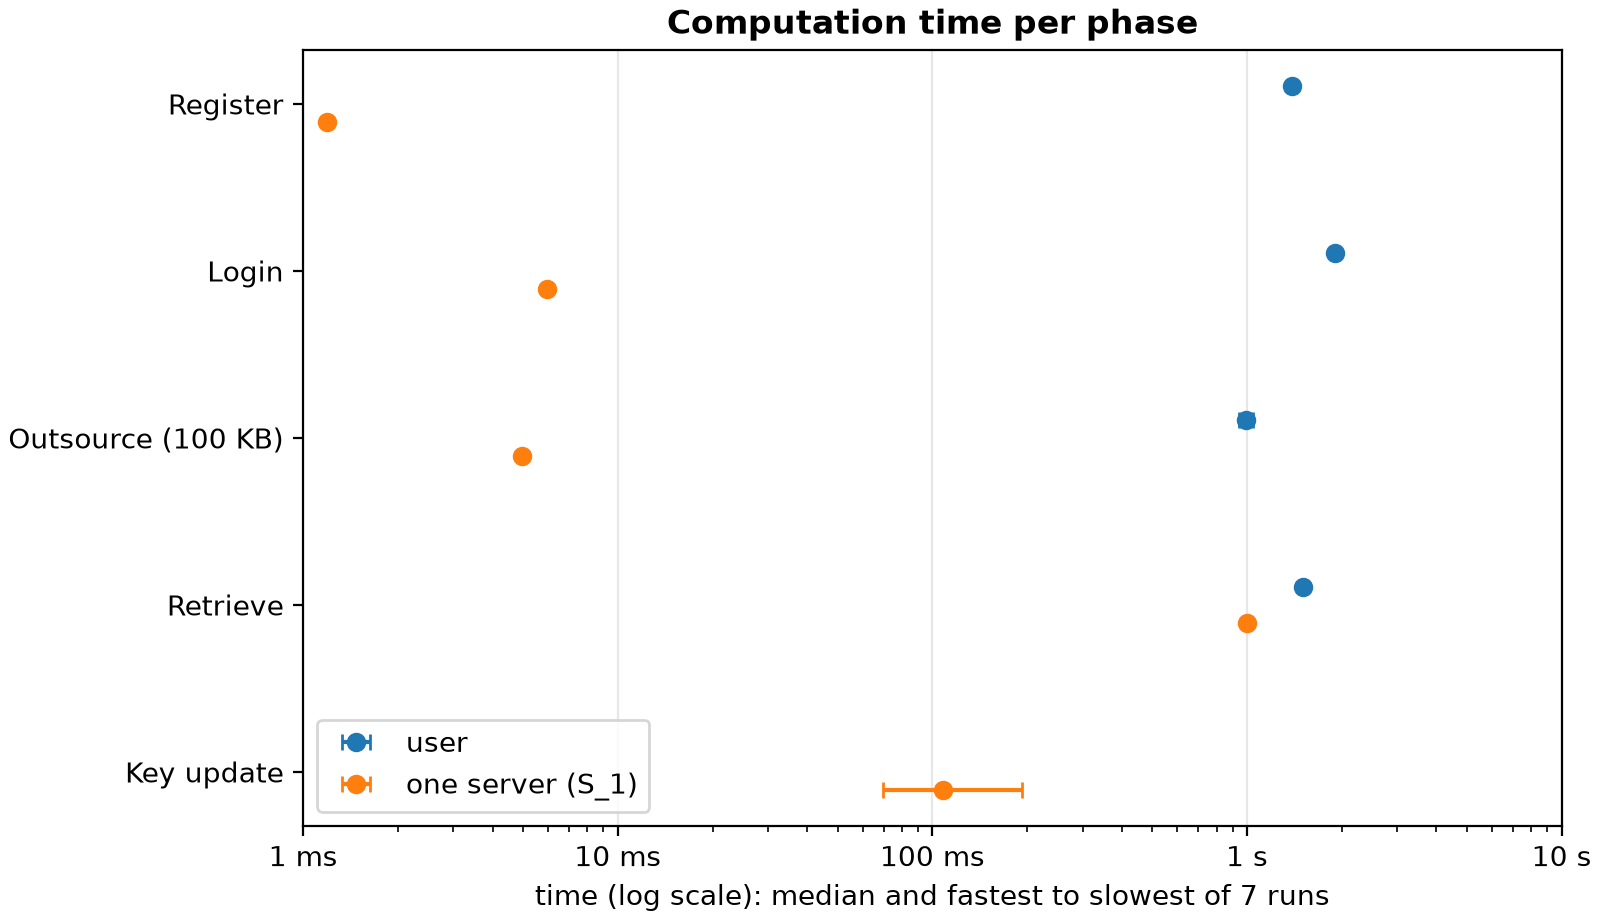
\includegraphics[width=0.86\linewidth]{phase_costs.png}
\caption{Computation time per phase at the user and at one server, on a log scale: the median of 7 runs and the
fastest to the slowest run. Drawn by \texttt{notebooks/05\_costs.ipynb}, cell 13.}
\label{fig:phase-costs}
\end{figure}

\begin{table}[ht]
\centering
\small
\caption{Building blocks. $a_x$ is one PRF chain, \cref{eq:bp-prf}. Source: \texttt{notebooks/05\_costs.ipynb},
cell 13.}
\label{tab:cost-blocks}
% generated by report/tools/make_numbers.py from notebooks/05_costs.ipynb, cell 13
\begin{tabular}{lrrr}
\toprule
\textbf{building block} & \textbf{median} & \textbf{range (min to max)} & \textbf{runs} \\
\midrule
a\_x & 492 ms & 490 ms to 496 ms & 7 \\
Ring.mul (ell, n) x (n,) & 0.67 ms & 0.66 ms to 0.71 ms & 31 \\
ML-DSA-44 keygen & 3.94 ms & 3.85 ms to 4.01 ms & 101 \\
ML-DSA-44 sign & 19.8 ms & 10.1 ms to 85.6 ms & 101 \\
ML-DSA-44 verify & 4.79 ms & 4.71 ms to 5.37 ms & 101 \\
AES-256-GCM encrypt 100 KB & 0.021 ms & 0.021 ms to 0.023 ms & 31 \\
AES-256-GCM decrypt 100 KB & 0.021 ms & 0.020 ms to 0.022 ms & 31 \\
linear hash H & 0.20 ms & 0.20 ms to 0.21 ms & 31 \\
TOPRF blind (U) & 1.15 ms & 1.14 ms to 1.17 ms & 7 \\
TOPRF evaluate (S\_i) & 1.09 ms & 1.09 ms to 1.10 ms & 7 \\
TOPRF combine (U) & 1.04 ms & 1.04 ms to 1.06 ms & 7 \\
\bottomrule
\end{tabular}

\end{table}

\begin{table}[ht]
\centering
\small
\caption{Each phase per party. ``PRF chains'' counts the lattice PRF evaluations in the phase. ``Share in PRF
chains'' divides the chain count times the $a_x$ time measured right after each run by that run's phase time, so it
can read slightly above 100\% when a phase is all PRF work. The limiter is the term of the cost model that takes the
largest share. Source: \texttt{notebooks/05\_costs.ipynb}, cell 13.}
\label{tab:cost-phases}
\resizebox{\linewidth}{!}{% generated by report/tools/make_numbers.py from notebooks/05_costs.ipynb, cell 13
\begin{tabular}{llrrrrl}
\toprule
\textbf{phase} & \textbf{party} & \textbf{median} & \textbf{range (min to max)} & \textbf{PRF chains} & \textbf{share in PRF chains} & \textbf{limiter (share of time)} \\
\midrule
Register & user & 1.39 s & 1.39 s to 1.40 s & 3 & 102\% & PRF chains a\_x (102\%) \\
Register & one server (S\_1) & 1.19 ms & 1.18 ms to 1.20 ms & 0 & 0\% & TOPRF evaluate (92\%) \\
Login & user & 1.90 s & 1.88 s to 1.91 s & 4 & 97\% & PRF chains a\_x (97\%) \\
Login & one server (S\_1) & 5.94 ms & 5.87 ms to 5.97 ms & 0 & 0\% & ML-DSA-44 verify (81\%) \\
Outsource (100 KB) & user & 994 ms & 943 ms to 1.05 s & 2 & 93\% & PRF chains a\_x (93\%) \\
Outsource (100 KB) & one server (S\_1) & 4.95 ms & 4.91 ms to 4.97 ms & 0 & 0\% & ML-DSA-44 verify (97\%) \\
Retrieve & user & 1.50 s & 1.49 s to 1.52 s & 3 & 92\% & PRF chains a\_x (92\%) \\
Retrieve & one server (S\_1) & 1000 ms & 998 ms to 1.00 s & 2 & 92\% & PRF chains a\_x (92\%) \\
Key update & one server (S\_1) & 108 ms & 69.6 ms to 193 ms & 0 & 0\% & ML-DSA-44 sign (68\%) \\
Key update & all 3 servers & 326 ms & 271 ms to 433 ms & 0 & 0\% & ML-DSA-44 sign (67\%) \\
\bottomrule
\end{tabular}
}
\end{table}

One number explains most of these times. A PRF chain, one evaluation of $a_x$, takes \AxMedian. Every HKDF and
PRF call in our implementation is a chain, and so is the password encoding in the TOPRF. The user's Register runs
three chains, Login four, Outsource two, and Retrieve three, and those chains account for at least
\ChainShareMin{} of each phase (\cref{tab:cost-phases}). A server runs no chain except in Retrieve, where it runs one for each item that matches
the query. That is why a server's Retrieve takes \CostRetrieveServer{} with two matching items, while its Login
takes \CostLoginServer, mostly one ML-DSA-44 verification at \CostVerifyMedian. The key update is dominated by
ML-DSA-44 signing (\CostSignMedian{} median). Encrypting a 100~KB document with AES-256-GCM takes only
\CostAesMedian.

\subsection{Comparison with the paper's reported costs}

\Cref{tab:paper-vs-ours} sets our medians next to the paper's Table IV. The paper measured a C++ implementation
with NTL on an AMD Ryzen 7 5800H, at PARAM~II with $N = t = 2$~\cite{jiang2024qpase}. We measured Python at
PARAM~I with $N = 3$ and $t = 2$. Our user-side Register and Login take about \RatioRegisterUser{} and
\RatioLoginUser{} times as long as the paper reports, and Outsource and Retrieve about \RatioOutsourceUser{} and
\RatioRetrieveUser{} times as long.

\begin{table}[ht]
\centering
\small
\caption{Time per phase: the paper's Table IV against our medians from \cref{tab:cost-phases}.}
\label{tab:paper-vs-ours}
\begin{tabular}{lrrrr}
\toprule
& \multicolumn{2}{c}{\textbf{User}} & \multicolumn{2}{c}{\textbf{Server}} \\
\cmidrule(lr){2-3}\cmidrule(lr){4-5}
\textbf{Phase} & \textbf{Paper} & \textbf{Ours} & \textbf{Paper} & \textbf{Ours} \\
\midrule
Register & 0.99 ms & \CostRegisterUser & 0.05 ms & \CostRegisterServer \\
Login (recover $\Ku$) & 0.64 ms & \CostLoginUser & 0.05 ms & \CostLoginServer \\
Outsource (100 KB) & 16.05 ms & \CostOutsourceUser & 0.13 ms & \CostOutsourceServer \\
Retrieve & 30.95 ms & \CostRetrieveUser & 15.69 ms & \CostRetrieveServer \\
\bottomrule
\end{tabular}
\end{table}

Part of the gap is the language: our ring products run through numpy from Python. Most of it is the PRF. The
paper's Table III lists one PRF evaluation at 0.554~ms and one HKDF evaluation at 0.02~ms; our chain takes
\AxMedian, about \RatioPrf{} times the paper's PRF figure. A full evaluation of \cref{eq:bp-prf} needs
$(L-1)\,\ell^2$ ring products, which is \RingProductsChain{} at $L = \ParamL$ and $\ell = \ParamEll$, and our
profile attributes most of the chain's time to those products. The paper names the lattice PRF of Banerjee and
Peikert for both functions (its Sections II-C and V) but gives no implementation detail. We infer that its PRF and
HKDF timings measure a smaller computation than a full chain; the cause is unknown to us. This matters for the conclusions: in our implementation the lattice PRF,
not the TOPRF or the signatures, sets the cost of every user-side phase.

\subsection{Communication cost}

\Cref{fig:traffic} and \cref{tab:cost-traffic} give the exact bytes each phase sends. The lattice vectors dominate.
Each of $b$, $b_{k_i}$ and $pk_i$ is \SizePublicVector, so Register sends three of them per server and Login three
per contacted server. Outsource is dominated by the 100~KB document itself, and Retrieve by the two matching
documents that come back.

\begin{figure}[ht]
\centering
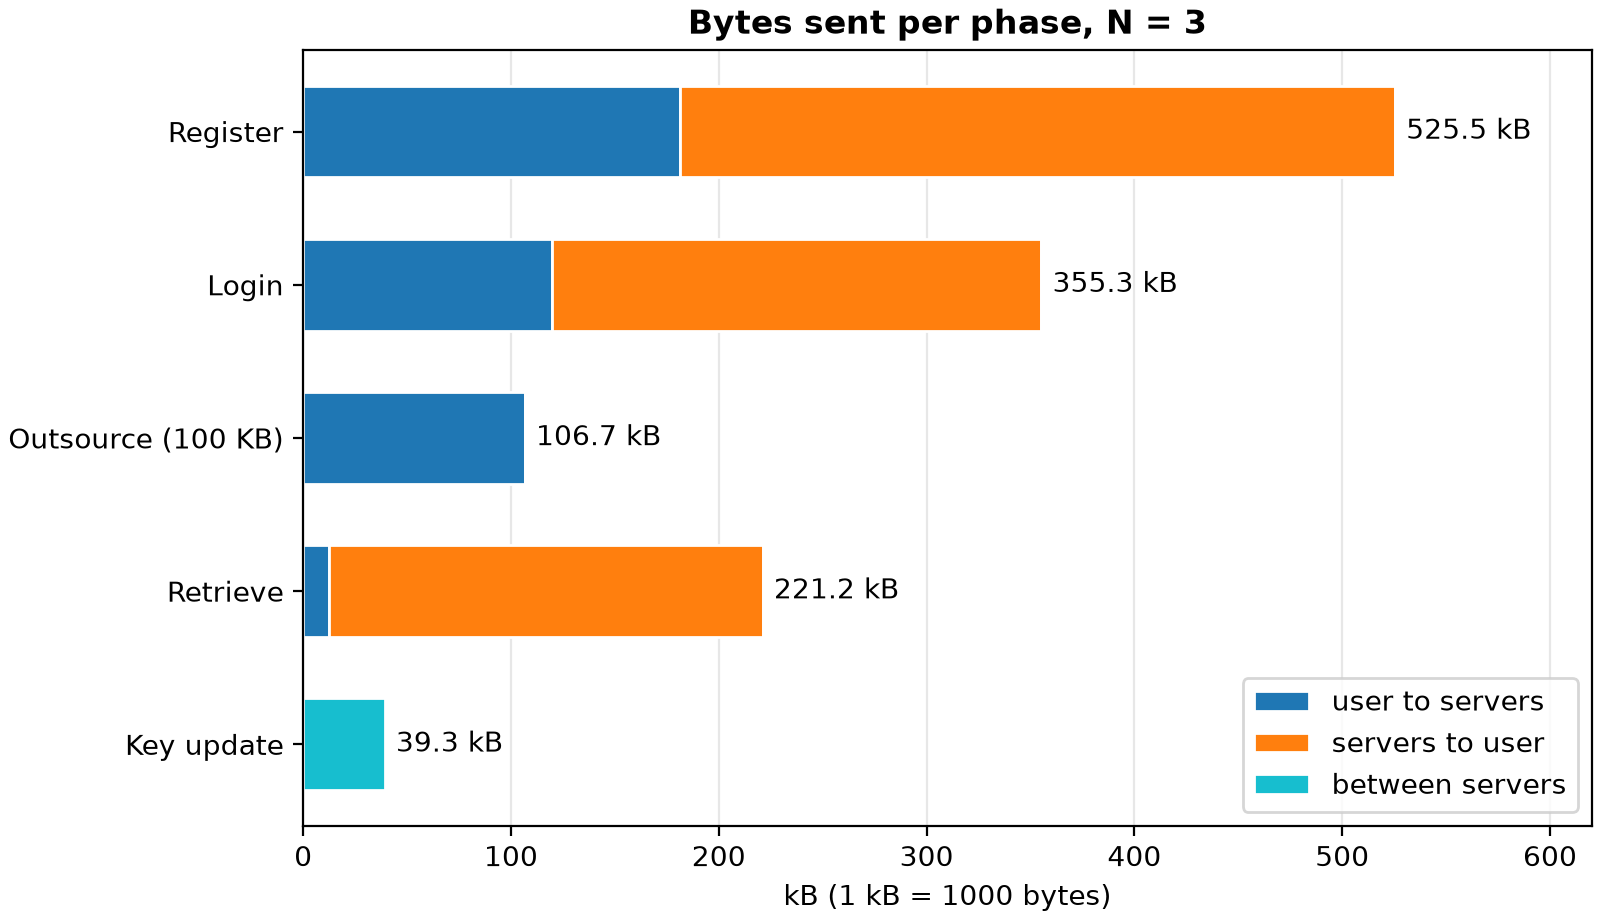
\includegraphics[width=0.86\linewidth]{traffic.png}
\caption{Bytes each phase sends, split by direction, with $N = 3$ servers. Drawn by
\texttt{notebooks/05\_costs.ipynb}, cell 13.}
\label{fig:traffic}
\end{figure}

\begin{table}[ht]
\centering
\small
\caption{Bytes per phase and direction, $N = 3$, $t = 2$, one 100~KB document per Outsource and two matching
documents per Retrieve. Source: \texttt{notebooks/05\_costs.ipynb}, cell 13.}
\label{tab:cost-traffic}
% generated by report/tools/make_numbers.py from notebooks/05_costs.ipynb, cell 13
\begin{tabular}{lrrrr}
\toprule
\textbf{phase} & \textbf{user to servers} & \textbf{servers to user} & \textbf{between servers} & \textbf{total} \\
\midrule
Register & 181398 B & 344064 B & 0 B & 525462 B \\
Login & 119612 B & 235648 B & 0 B & 355260 B \\
Outsource (100 KB) & 106709 B & 0 B & 0 B & 106709 B \\
Retrieve & 12645 B & 208568 B & 0 B & 221213 B \\
Key update & 0 B & 0 B & 39264 B & 39264 B \\
\bottomrule
\end{tabular}

\end{table}

The paper's Table IV reports about 4{,}404{,}019 bits for Register and 2{,}097{,}152 bits for recovering $\Ku$,
roughly 550~kB and 262~kB, with $N = t = 2$. Our Register (\TrafficRegister, $N = 3$) and Login (\TrafficLogin,
$t = 2$) are of the same order. For Outsource and Retrieve the paper reports about 111{,}332 and 119{,}050 bits.
111{,}332 bits is 13.9~kB, less than the 100~KB file being outsourced, so we read these two figures as bytes; the
paper does not say. In bytes they agree with our Outsource of \TrafficOutsource.

\subsection{Security findings}
\label{sec:findings}

\subsubsection{PARAM II in the ring \texorpdfstring{$\mathbb{Z}_q[X]/(X^{595}+1)$}{Z\_q[X]/(X\^{}595+1)} allows offline password guessing}
\label{sec:param-ii}

Table II gives PARAM~II the degree $n = 595$. We run it in the ring of the scheme text, $\Rq = \mathbb{Z}_q[X]/(X^n+1)$
(\cref{sec:decisions}). Because 595 is odd, $(-1)^{595} + 1 = 0$, so $X = -1$ is a root of $X^{595}+1$, and
evaluating a polynomial at $-1$,
\[
\varphi(a) = a(-1) = \sum_i (-1)^i a_i \bmod q,
\]
is a ring homomorphism from $\Rq$ to $\mathbb{Z}_q$. It turns each ring-LWE sample into a one-dimensional sample
that is easy to solve. A server that receives one blinded TOPRF request $b = a r + a_x + 2e$ can test a password
guess $x'$ offline. It computes $c_j = \varphi(b_j) - \varphi(a_{x',j}) = \varphi(a_j)\varphi(r) + 2\varphi(e_j) +
\varphi(a_{x,j} - a_{x',j})$ for each of the $\ell$ entries. For the right guess the last term vanishes, and
$\varphi(r)$ and $\varphi(e_j)$ are sums of 595 small Gaussians, about $\sigma\sqrt{n} = \ParamIISigmaSqrtN$ in size.
The server tries every $\rho$ with $|\rho| \le \ParamIIRadius$ and keeps the guess if $c_j - \rho\,\varphi(a_j)$ is
small in every entry. A wrong guess leaves the last term uniform in $\mathbb{Z}_q$, so no $\rho$ fits.

\begin{figure}[ht]
\centering
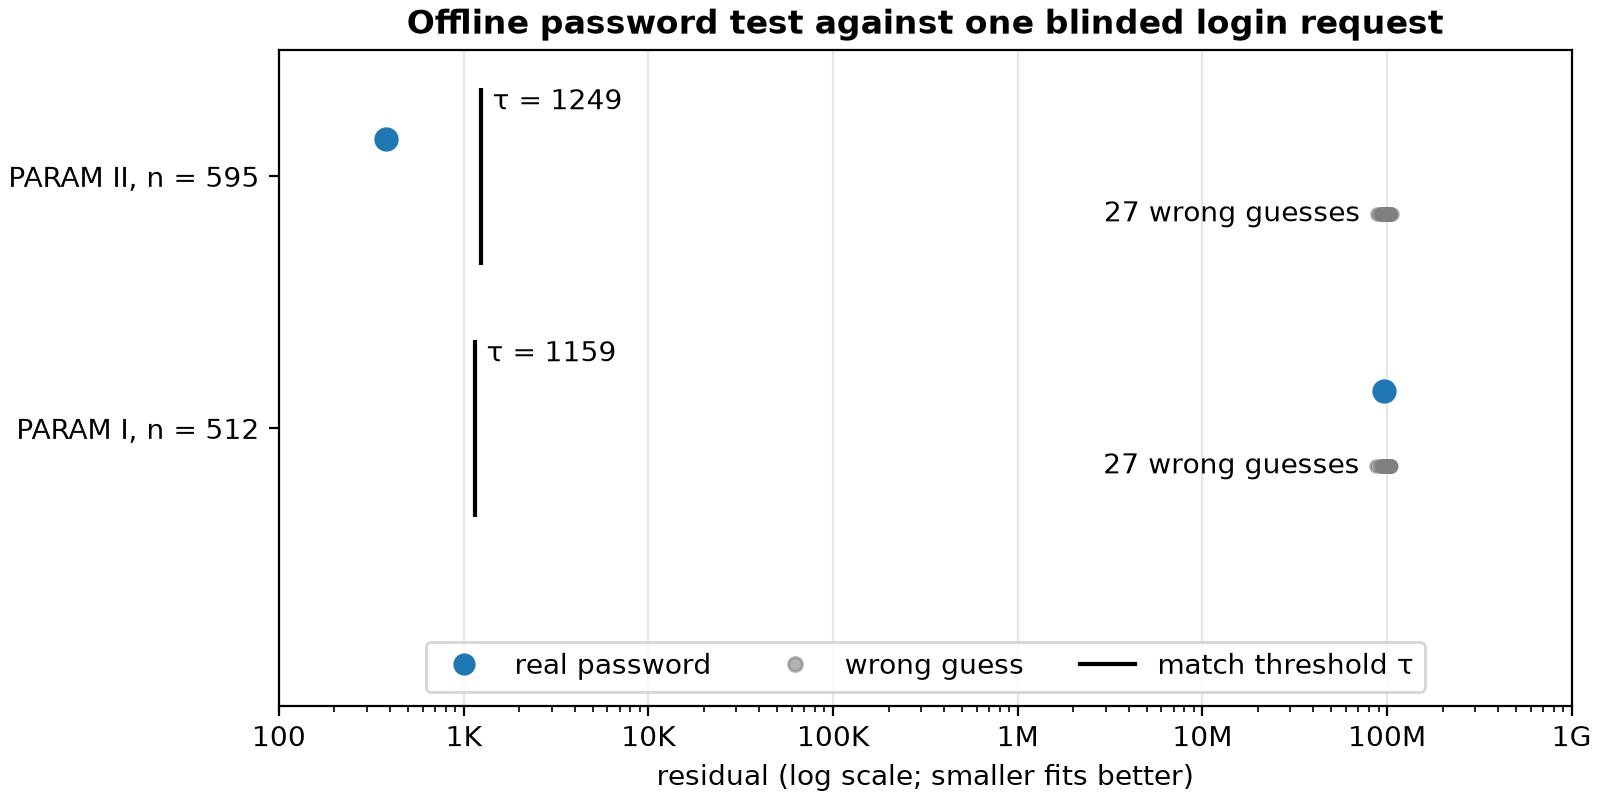
\includegraphics[width=0.82\linewidth]{param_ii_residuals.png}
\caption{Residual of each of \ParamIIGuesses{} guesses against one blinded login request. Below the threshold
$\tau$ a guess matches. Drawn by \texttt{notebooks/06\_param\_ii\_offline\_guessing.ipynb}, cell 7.}
\label{fig:param-ii}
\end{figure}

\begin{table}[ht]
\centering
\small
\caption{The offline test against one request. Source:
\texttt{notebooks/06\_param\_ii\_offline\_guessing.ipynb}, cell 7.}
\label{tab:param-ii}
\resizebox{\linewidth}{!}{% generated by report/tools/make_numbers.py from notebooks/06_param_ii_offline_guessing.ipynb, cell 7
\begin{tabular}{lrrrrl}
\toprule
\textbf{parameter set} & \textbf{threshold tau} & \textbf{real password residual} & \textbf{smallest wrong-guess residual} & \textbf{largest wrong-guess residual} & \textbf{guesses matched} \\
\midrule
PARAM II, n = 595 & 1249 & 382 & 88243150 & 106898851 & sunshine1 \\
PARAM I, n = 512 & 1159 & 96673162 & 87519736 & 105468868 & none \\
\bottomrule
\end{tabular}
}
\end{table}

Notebook~06 runs the test over a dictionary of \ParamIIGuesses{} common passwords that contains the real one
(\cref{fig:param-ii,tab:param-ii}). At PARAM~II the real password leaves a residual of \ParamIITrueResidual, below
the threshold $\tau = \ParamIITau$, and every wrong guess leaves at least \ParamIIMinWrong. The whole dictionary
took \ParamIIAttackTime. At PARAM~I, $X^{512}+1$ has no root modulo $q$, and nothing matches: the real password's
residual (\ParamIReal) is as large as the wrong guesses'. The attack breaks the resistance to offline guessing, the
first attack in the paper's threat model, for PARAM~II as we run it. The paper's security estimate for $n = 595$
probably assumes plain LWE, where this attack does not apply, so the flaw belongs to our reading of the parameters
and is not proven of the paper. All other experiments therefore use PARAM~I.

\subsubsection{The linear key-update commitments reveal the shares}

Step 4 of the key update checks $H(F_{ji}) = \sum_k i^k H(\alpha_k)$, which requires $H$ to be linear. We use
$H(x) = A_H x \bmod q$ with a square matrix $A_H$ expanded from SHAKE256. A random square matrix modulo the prime
$q$ is invertible with overwhelming probability, and ours is: \texttt{report/tools/invert\_commitment.py} solves
$A_H x = h$ by Gaussian elimination modulo $q$ and recovers a random $\alpha$ from its commitment $H(\alpha)$
exactly. This check runs outside the notebooks. The broadcast commitments $h_k = H(\alpha_k)$ therefore reveal
each $\alpha_k$, hence every share $F_{ji}$ and every key change $k'_i - k_i$, to anyone who sees them. The update
no longer protects a key share that leaked in an earlier epoch. Another linear $H$ only moves the problem. An
injective $H$ can be inverted in the same way. A compressing $H$ hides part of $\alpha_k$, but then a dealer can
add a vector from its kernel and change a share without changing $H$, so the commitment no longer binds. The shares still verify and $K$ still stays the same, but a fix needs a hiding commitment with randomness,
which the paper does not specify.
